%!TEX root = main.tex
\section{Participatory Design Findings}
From participatory design, we learned about the characteristic problems and challenges present to VQSs and identified key features that addresses these challenges. Based on feature requests and discussion with our participants, we incorporated key features missing in our original VQS.
%From these discussion and analysis of past VQSs, we identify nine components of VQSs, described below. T
Along with analysis of past literature, we develop a taxonomy based on the features organized as components. These components are then organized into three paradigms of sensemaking in VQSs that span across different areas in the design space. As presented in this section, our study is the first that contributes towards a holistic understanding of the sensemaking process for visual querying.
% novel contribution on  ---
% contribute to holistic understanding on how sensemaking --- in VQS.
% study on how users
% Implication ---
% •	What types of questions/ dataset/ problem challenges are asked to VQS or can be addressed by VQS? (S3)
% •	What kind of features needs to be designed to address these challenges (S4 PD)
%We employed participatory design with our scientists to incorporate key features missing in our original VQS, and unaddressed in their existing workflows. From these discussion and analysis of past VQSs, we identify nine components of VQSs, described below.
\subsection{Themes Emerging from Participatory Design\label{sec:pd_findings}}
\begin{figure*}[t!]
\centering
\vspace{-15pt}
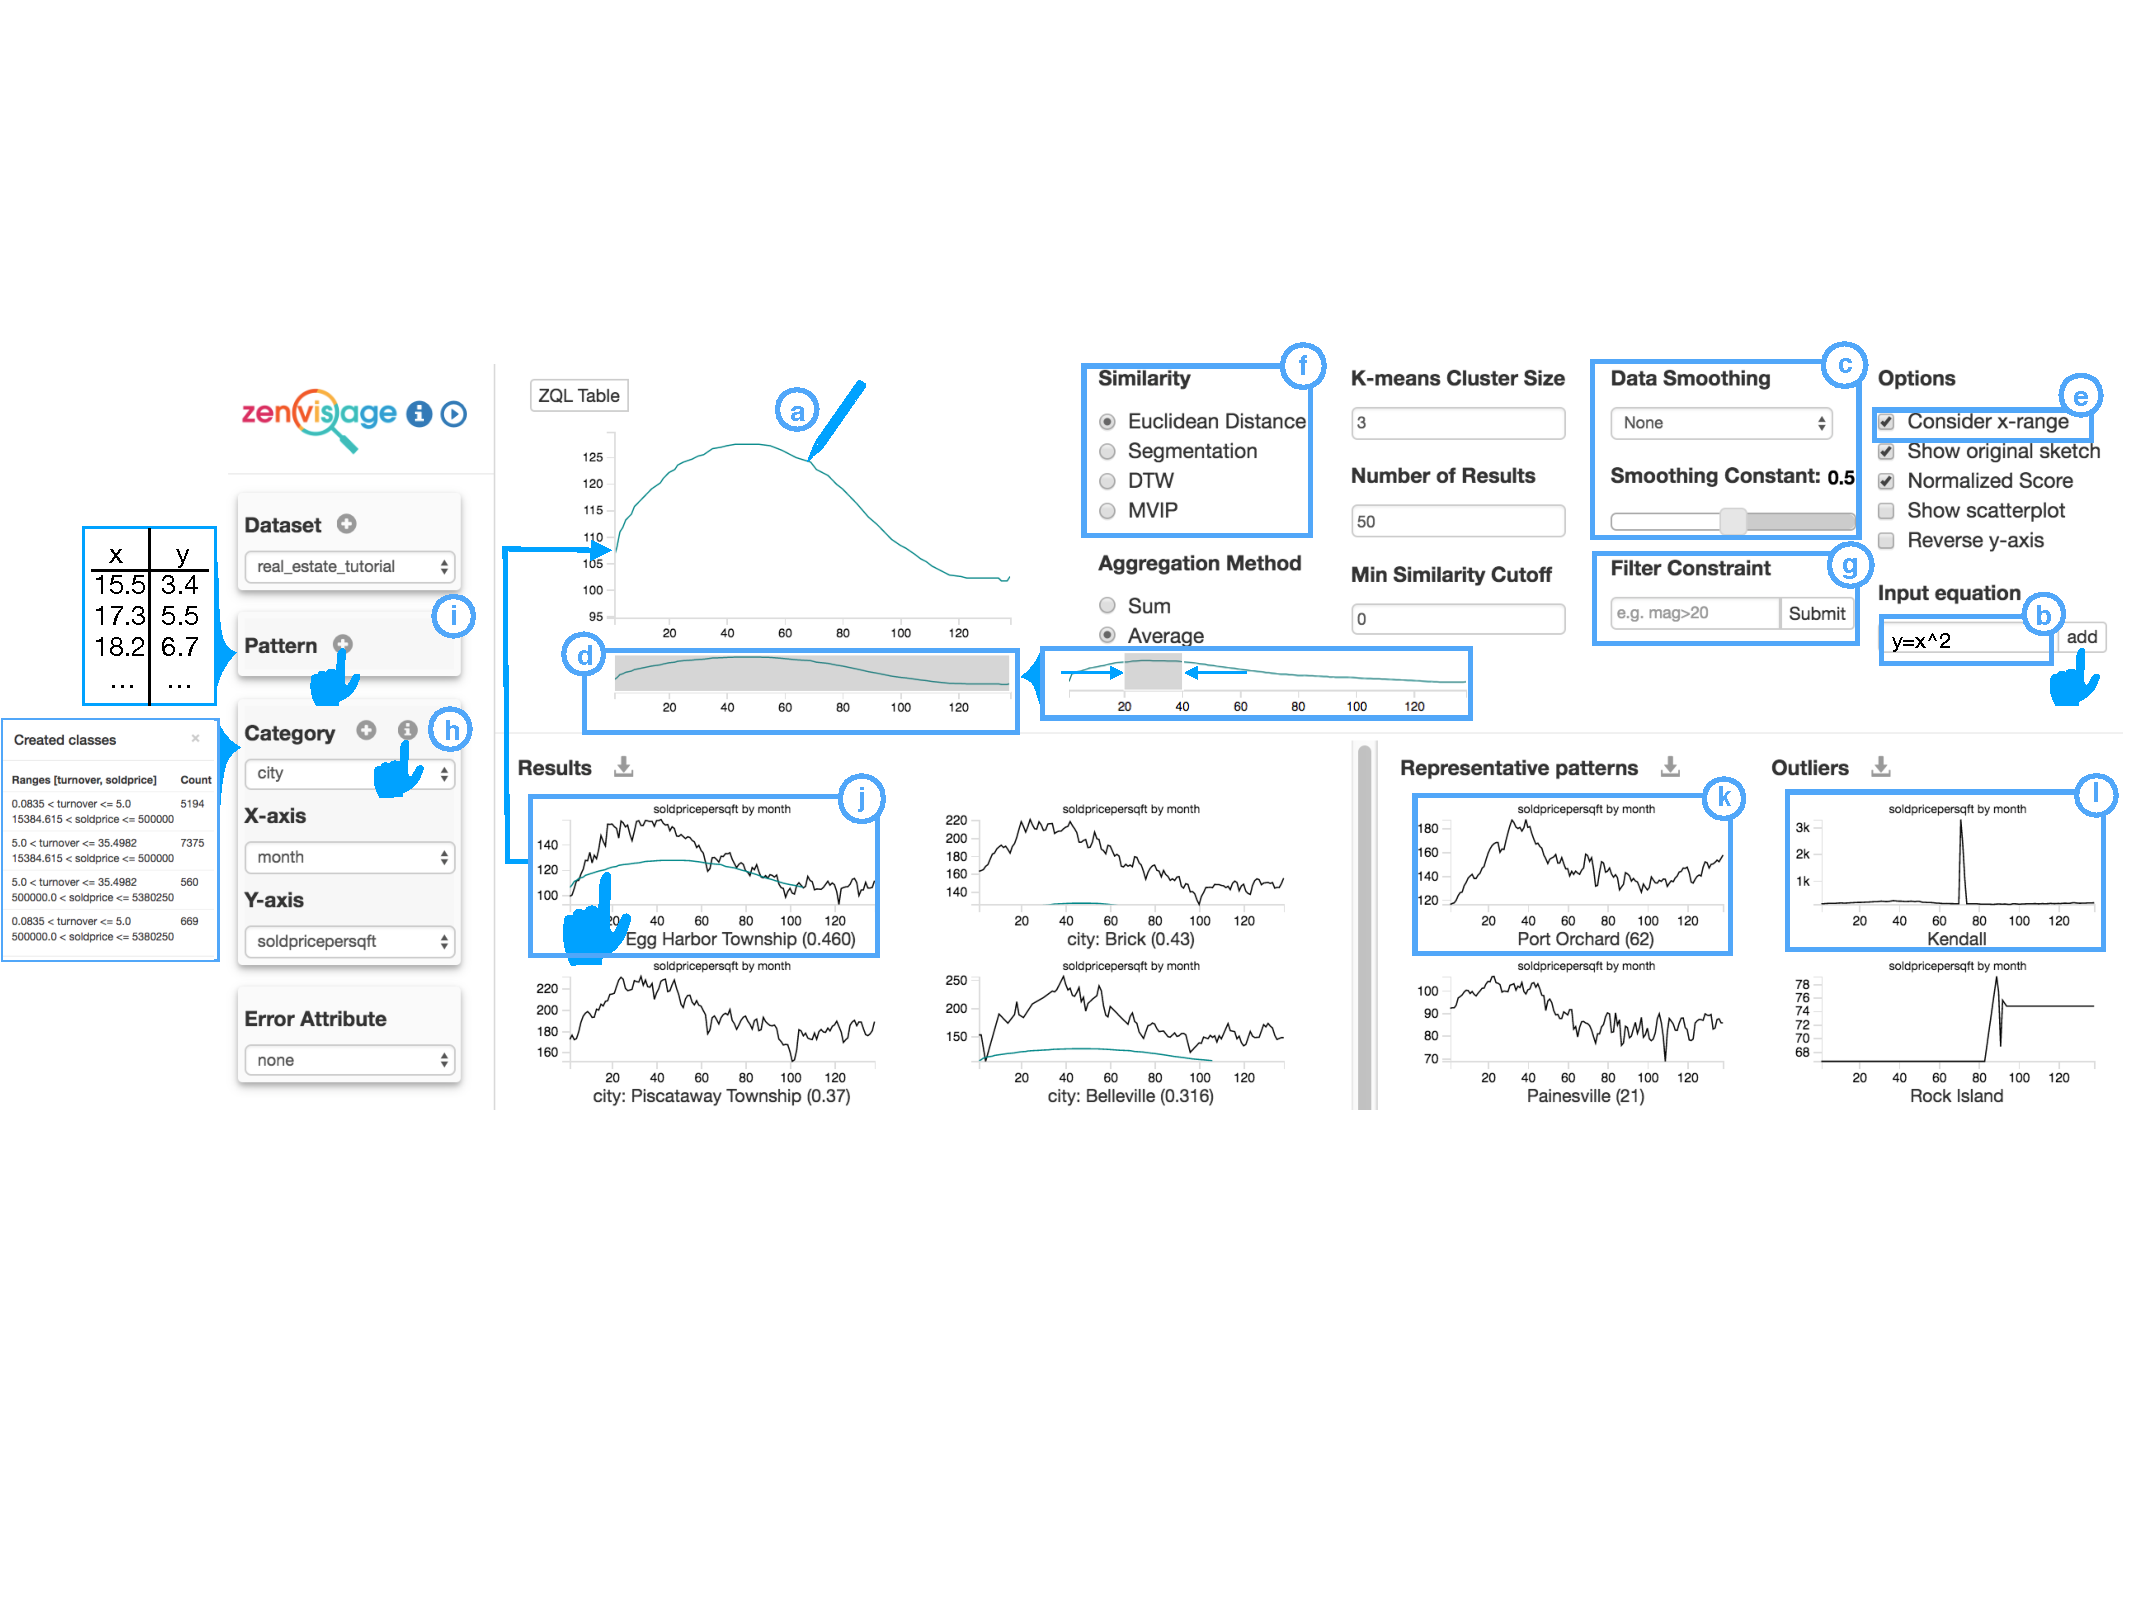
\includegraphics[width=\linewidth]{figures/system.pdf} %5.5
\vspace{-5pt}\caption{Our VQS after participatory design, which includes: the ability to query via (a) a sketch,(b) input equations, (i) drag and drop, or (j) uploaded patterns; (c) preprocessing via data smoothing; query specification mechanisms including (d) x-range selection and filtering, (e) x-range invariance, (g) Filtering, and (h) Dynamic class creation; recommendation of (k) representative and (l) outlier trends. Prior to the participatory design, \zv only included a single sketch input with no additional options.}
\label{zvOverview}
\vspace{-14pt}
\end{figure*}

 %We discovered three central themes encapsulating these features that are important to facilitate rapid hypothesis generation and insight discovery, but are missing in prior VQSs. While some of our findings echo prior work on system-level taxonomies of visualization tasks \cite{Amar2005,Heer2012}, we highlight how specific analytic tasks and interaction features could be used to enhance VQSs in particular. \techreport{In particular, we learned that \textit{participants wanted more control over the internals of the systems and an integrated workflow that helped streamline their analysis when using VQSs.}}
\boldpara{Exact Shape Specification} interfaces allow users to submit a query through an exact description of a pattern, then the VQS returns a list of most similar matches. Almost all VQS supports freehand sketching \techreport{on a virtual canvas through mouse or pen as a intuitive mechanism }for specifying desired patterns (Figure \ref{zvOverview}a). In addition to sketching, \zv also allows users to specify a functional form (e.g. y=$x^2$) for a pattern (Figure \ref{zvOverview}b). This feature was inspired by material scientists who were interested in finding solvents with known analytical models that describes the relationships between their chemical properties.
\boldpara{Approximate Shape Specification:} While exact shape specification is an intuitive mechanism for constructing a visual query, as pointed out by past works~\cite{correll2016semantics,Holz2009}, pattern queries can be extremely imprecise. Many interfaces have developed constrained sketching mechanism to allow users to partially specify certain characteristics, such as angular slope queries for specifying the slope of a trend line~\cite{Hochheiser2004} or piecewise trend querylines over a specified data range~\cite{ryall2005querylines}. Both Qetch and \zv supports data smoothing to allow users to interactively change the degree of shape approximation they would like to apply to all visualizations (and consequently for pattern matching). Motivated by the dense and noisy observational data in the astronomy and material science use cases, we developed an interface for users to interactively adjust data smoothing algorithm and parameters on-the-fly to update the resulting visualizations accordingly (Figure \ref{zvOverview}c).
\techreport{\par During participatory design, both material science and astronomy participants noted the difficulty of shape matching on their dense and noisy observational data and the challenge of picking the appropriate smoothing parameters during offline preprocessing. We found that tight integration between smoothing and visual search additionally tradeoff between the smoothness of the curve and the degree of approximation for shape-matching in VQSs. An over-smoothed visualization would return shape matches that only loosely resemble the query pattern. However, without smoothing, the noise may dominate the overall trend, which could lead to bad pattern matches.}
%While the interactions in our original prototype enabled simple visual queries, many scientists were interested in extending their querying capabilities, either through different querying modalities or through more flexible query specification methods.

% While \zv does not attempt to solve all of the pre-processing issues that we faced during participatory design, we identified data smoothing as a common data cleaning procedure that could benefit from a tight integration between pre-processing and visual analysis. Data smoothing is a denoising procedure that generates a smoothed pattern approximating key features of the visualized trend with less noise.
\boldpara{Range Selection:} Often in time series analysis there are specific ranges of time and measure values with special domain specific significance that may be of interest to users. One common specification is to limit the pattern query to be matched only in specific x or y ranges. Range selection can be performed through explicit textbox specification~\cite{wattenberg2001sketching,Mannino2018}, drawing line limits~\cite{ryall2005querylines}, or brushing interactions~\cite{Hochheiser2001}. \zv employs the brushing mechanism to select desirable x-ranges to perform shape matching (Figure \ref{zvOverview}d). Additionally, y axis range selection could be performed through entering a filter constraint on the measure variable.
\par We chose to support only brushing for x, since it was more common to focus the context based on the independent variable in our use cases, such as zooming into particular sharp dips when looking for planetary transits or anomalous peaks indicative of erroneous experimental measurements. \cut{In contrast, y-range selection tends to be more global and enforced across multiple interaction sequences, such as looking for only signals above a certain threshold.} The TimeSearcher and Queryline approach is most flexible for range selection as they allow composition of multiple range selection to formulate complex piecewise queries, such as finding a gene expression profile rising from x=1-5 then declining from x=5-10.
\boldpara{Flexible Matching:} Studies have shown that to facilitate subjectively meaningful pattern matches, VQSs need to support mechanisms for clarifying sketch interpretation and flexible shape matching algorithms~\cite{correll2016semantics,Mannino2018,Eichmann2015}. In \zv, users have the option to change similarity metrics that perform flexible matching (Figure \ref{zvOverview}e), as well as the option to ignore the x-range in shape matching (Figure \ref{zvOverview}f). For finding supernovae, A1 primarily cared about the existence of a peak above a certain amplitude with an appropriate width of the curve, rather than the exact time that the event occurred. G1 also expressed that she does not care about when the ``trigger point'' is as long as the profile is ``rising''. This latter features is akin to the temporal invariants in SketchQuery.

\boldpara{Filter Selection:} We find that users with large datasets often need to first use domain knowledge to narrow down their search to a subset of data. This increases their chances of finding an interesting pattern for a given pattern query. To filter data on-the-fly in \zv, users could compose one or more conditions as filter constraints in a text field (Figure \ref{zvOverview}g). \cut{The filtering can be done on data columns associated with each pattern that is not visualized or on the visualized attributes. This feature is unique to \zv as most existing VQSs do not allow users to interact with data in the non-visualized columns.}
%We designed two dynamic faceting features coupled with coordinated views that enabled users to specify subsets of data they are querying on and see immediate changes updated in the query, representative, and outlier results.
\boldpara{Group Comparison} addresses a common analytical question from our participatory design where users want to bucket data points into customized classes based on existing properties, and subsequently compare between the customized classes. For example, M1 wanted to create classes of solvents with ionization potential under -10 kJ/mol, over -8 kJ/mol, and ones between that range. Then, he could browse how visualizations involving lithium solvation energy varied across the three classes. To this end, we implemented dynamic class creation, a feature that allows users to use multiple properties to create custom classes on-the-fly, effectively slicing-and-dicing the data based on their needs (Figure \ref{zvOverview}h). The information regarding the created classes is displayed in the dynamic class information table and as a tooltip over the aggregated visualizations.
% , as shown in Figure~\ref{dcc}.
% \begin{figure}[h!]
% \centering
% 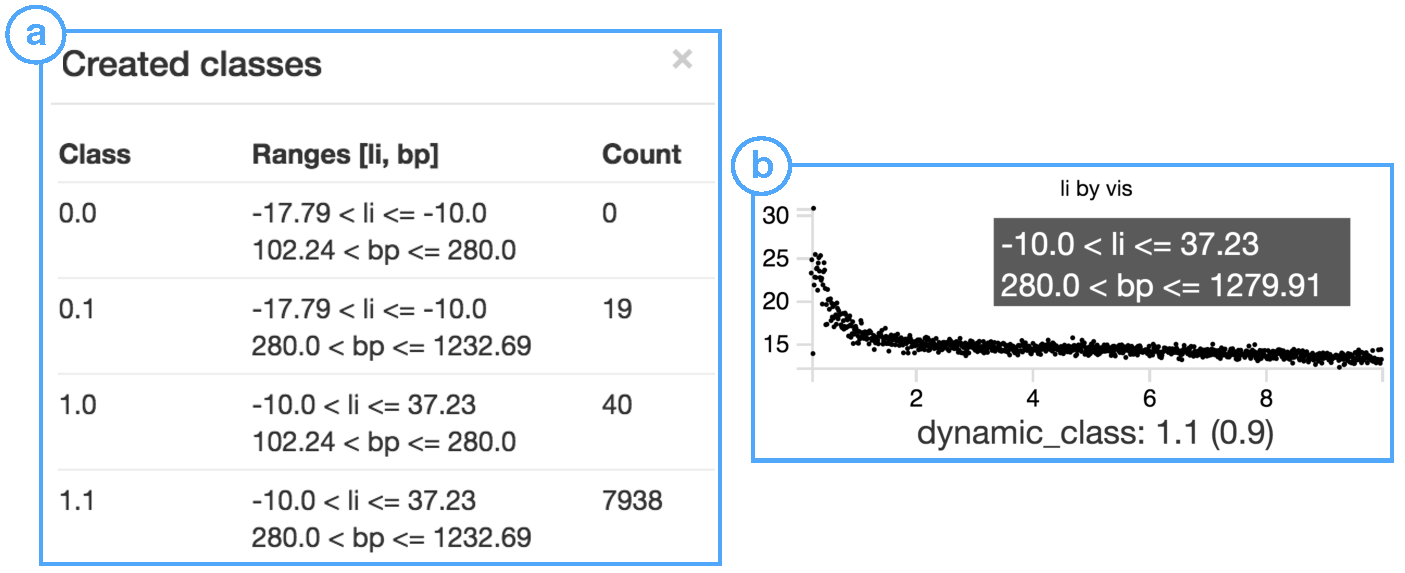
\includegraphics[width=\linewidth]{figures/dcc_example.pdf}
% \vspace{-6pt}
% \caption{Example of dynamic classes. (a) Four different classes with different Lithium solvation energies (li) and boiling point (bp) attributes based on user-defined data ranges. (b) Users can hover over the visualizations for each dynamic class to see the corresponding attribute ranges for each class. The visualizations of dynamic classes are aggregate across all the visualizations that lie in that class based on the user-selected aggregation method.}
% \label{dcc}
% \vspace{-10pt}
% \end{figure}
%While input equations are useful when simple analytical models exist, this may not be true for other domains. In these scenarios, users can upload a query pattern of a sequence of points
\boldpara{Concept querying} enable users to upload a pattern associated with a cconcept as a query. As supported in \zv and Google Correlate, users can upload a sequence of points as the query pattern (Figure \ref{zvOverview}i). This is useful for patterns generated from advanced computational models or prelabelled data from an external reference database. For example, A1 wanted to upload a query pattern based on synthetic light curves generated from simulations or known supernovae that have been discovered in the past. %Similarly, Google Correlate allows users to upload their own time series or enter search keywords that corresponds to a time series.
%, usually as part of the downstream analysis of the exploratory workflow. %For example, the genetics team are trying to develop a time series prediction algorithm using machine learning based on some biological parameters \cite{Peng2016}.
\boldpara{Result querying} allows users to submit a query based on the results, essentially asking for patterns that are similar to the selected data pattern. TimeSearcher enable users to instantiate queries via drag-and-drop, whereas QuerySketch does so similarly through double clicking. Similarly in \zv, users can drag and drop a visualization in either the results pane or the representative and outliers to the query canvas (Figure \ref{zvOverview}j). The distinction between concept and result querying is that concept querying loads in data external to the dataset, whereas result querying initiates the query using visualizations created from the queried data source.
\boldpara{Recommendation} displays visualizations that may be of interest to the users based on the data context. The recommendation feature is unique to \zv, which provides visualizations of representative trends based on clustering and highlights outlier instances that looks different from the rest of the visualizations (Figure \ref{zvOverview}k,l).
% In this section, we first describe a model to help characterize the design space for VQS based on the analytical workload and usage patterns from different use cases. Then, we present design challenges related to each of the process.
\subsection{Characterizing Design Space for VQSs}
Based on example use cases and feature components from our participatory design, we further characterize the design space of VQSs. Visual querying often consists of searching for a desired visualization instance across a visualization collection (Z) for some visualization axes (X,Y). We introduce two axes depicting the amount of information known about visualized attribute and pattern instance, as shown in Figure~\ref{2dmodel}.
\begin{figure}[h!]
  \centering
  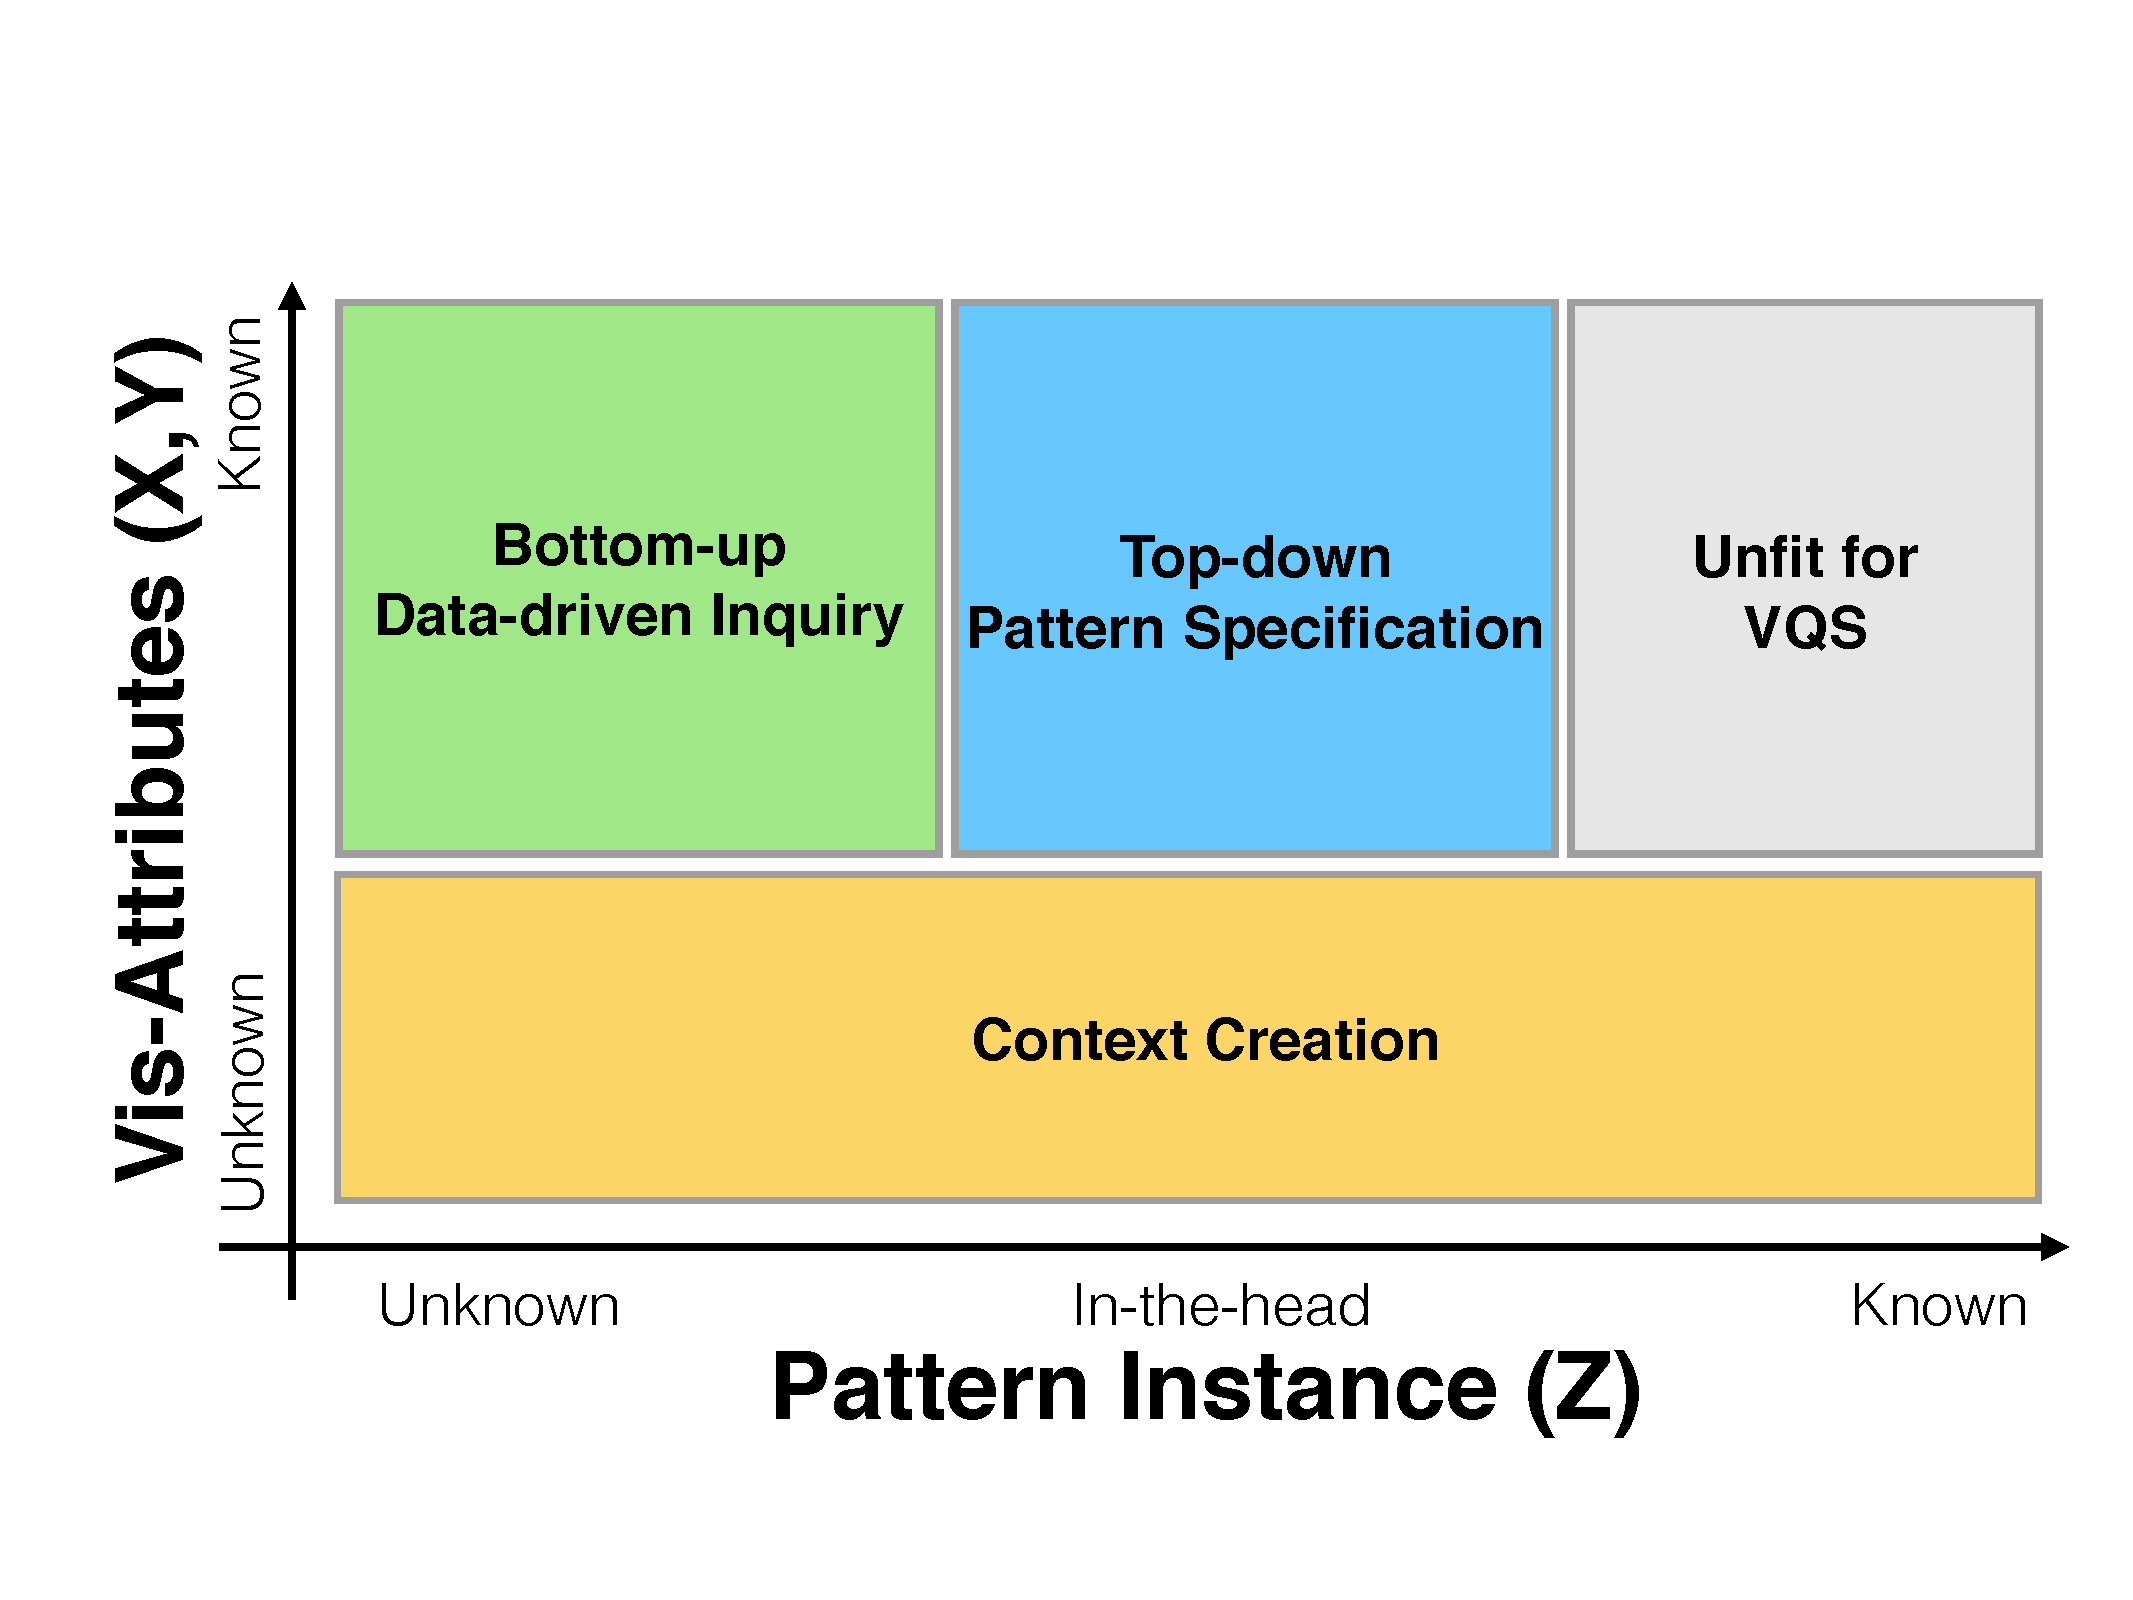
\includegraphics[width=\linewidth]{figures/2dmodel.pdf}
  \caption{The design space of VQSs is characterized by how much the analyst knows about the visualized attributes and pattern instance. Colored area highlights the three different paradigms of VQSs. While prior work has narrowed the focus of VQSs for use cases solely in the blue region, we envision opportunities for VQSs beyond this to a larger space of use cases and problems covered also by the red and green regions.}
  \dor{Should I take out the which, what, where and arrows in this Figure so it is less messy?}
  \label{2dmodel}
\end{figure}
\par Along the \textbf{pattern instance} axis, the visualization that contain the desired pattern may already be \texttt{known} to the analyst, exist as a pattern \texttt{in-the-head} of the analyst, or completely \texttt{unknown} to the analyst. For example, in the \texttt{known} pattern instance region (Figure~\ref{2dmodel} grey), a user wants to study only the pattern related to a specific gene. This use cases would be more suited for a visualization-at-a-time system, where analyst manually create and examine each visualization one at a time, rather than a VQS, since analysts can directly work with the selected instance without the need for visual querying. Inspired by Pirolli and Card's information foraging framework~\cite{Pirolli}, which distinguishes between information processing tasks that are \textit{top-down} (from theory to data) and \textit{bottom-up} (from data to theory), we define \textit{top-down pattern specification} as the search-oriented paradigm where analysts query based on their in-the-head pattern (Figure~\ref{2dmodel} blue). On the other hand, in the realm of \textit{bottom-up data-driven inquiry} (Figure~\ref{2dmodel} red), the pattern of interest is unbeknownst and external to the user and must be driven by recommendations or queries that originate from the data (or equivalently, the visualization). As we will discuss latter, this process is a crucial but understudied topic in past works on VQSs.
%analysts often do not start with a known pattern instance. T
\par The second axis, \textbf{visualized attributes}, depicts how much the analyst knows about which X and Y axes she is interested in visualizing. Both the astronomy and genetics use cases, as well as past work in this space, had data in the form of a time series with \texttt{known} visualized attributes. In the case of our material science participants, they wanted to explore relationships between different X and Y variables. In the realm of \texttt{unknown} attributes, context creation (Figure~\ref{2dmodel} green) is essential for allowing users to pivot across different visualization subspaces. %Most past VQSs assume that the analyst has a desired pattern in-the-head that could be conveyed through visual specification, such as a sketch.
\subsection{Design Goals and Challenges for VQS Paradigms}
We further explore the design objectives and challenges of each paradigm by developing a taxonomy for organizing how various components fits into the paradigms, as shown in Figure~\ref{fig:taxonomy}.
\begin{figure*}[ht!]
  \centering
  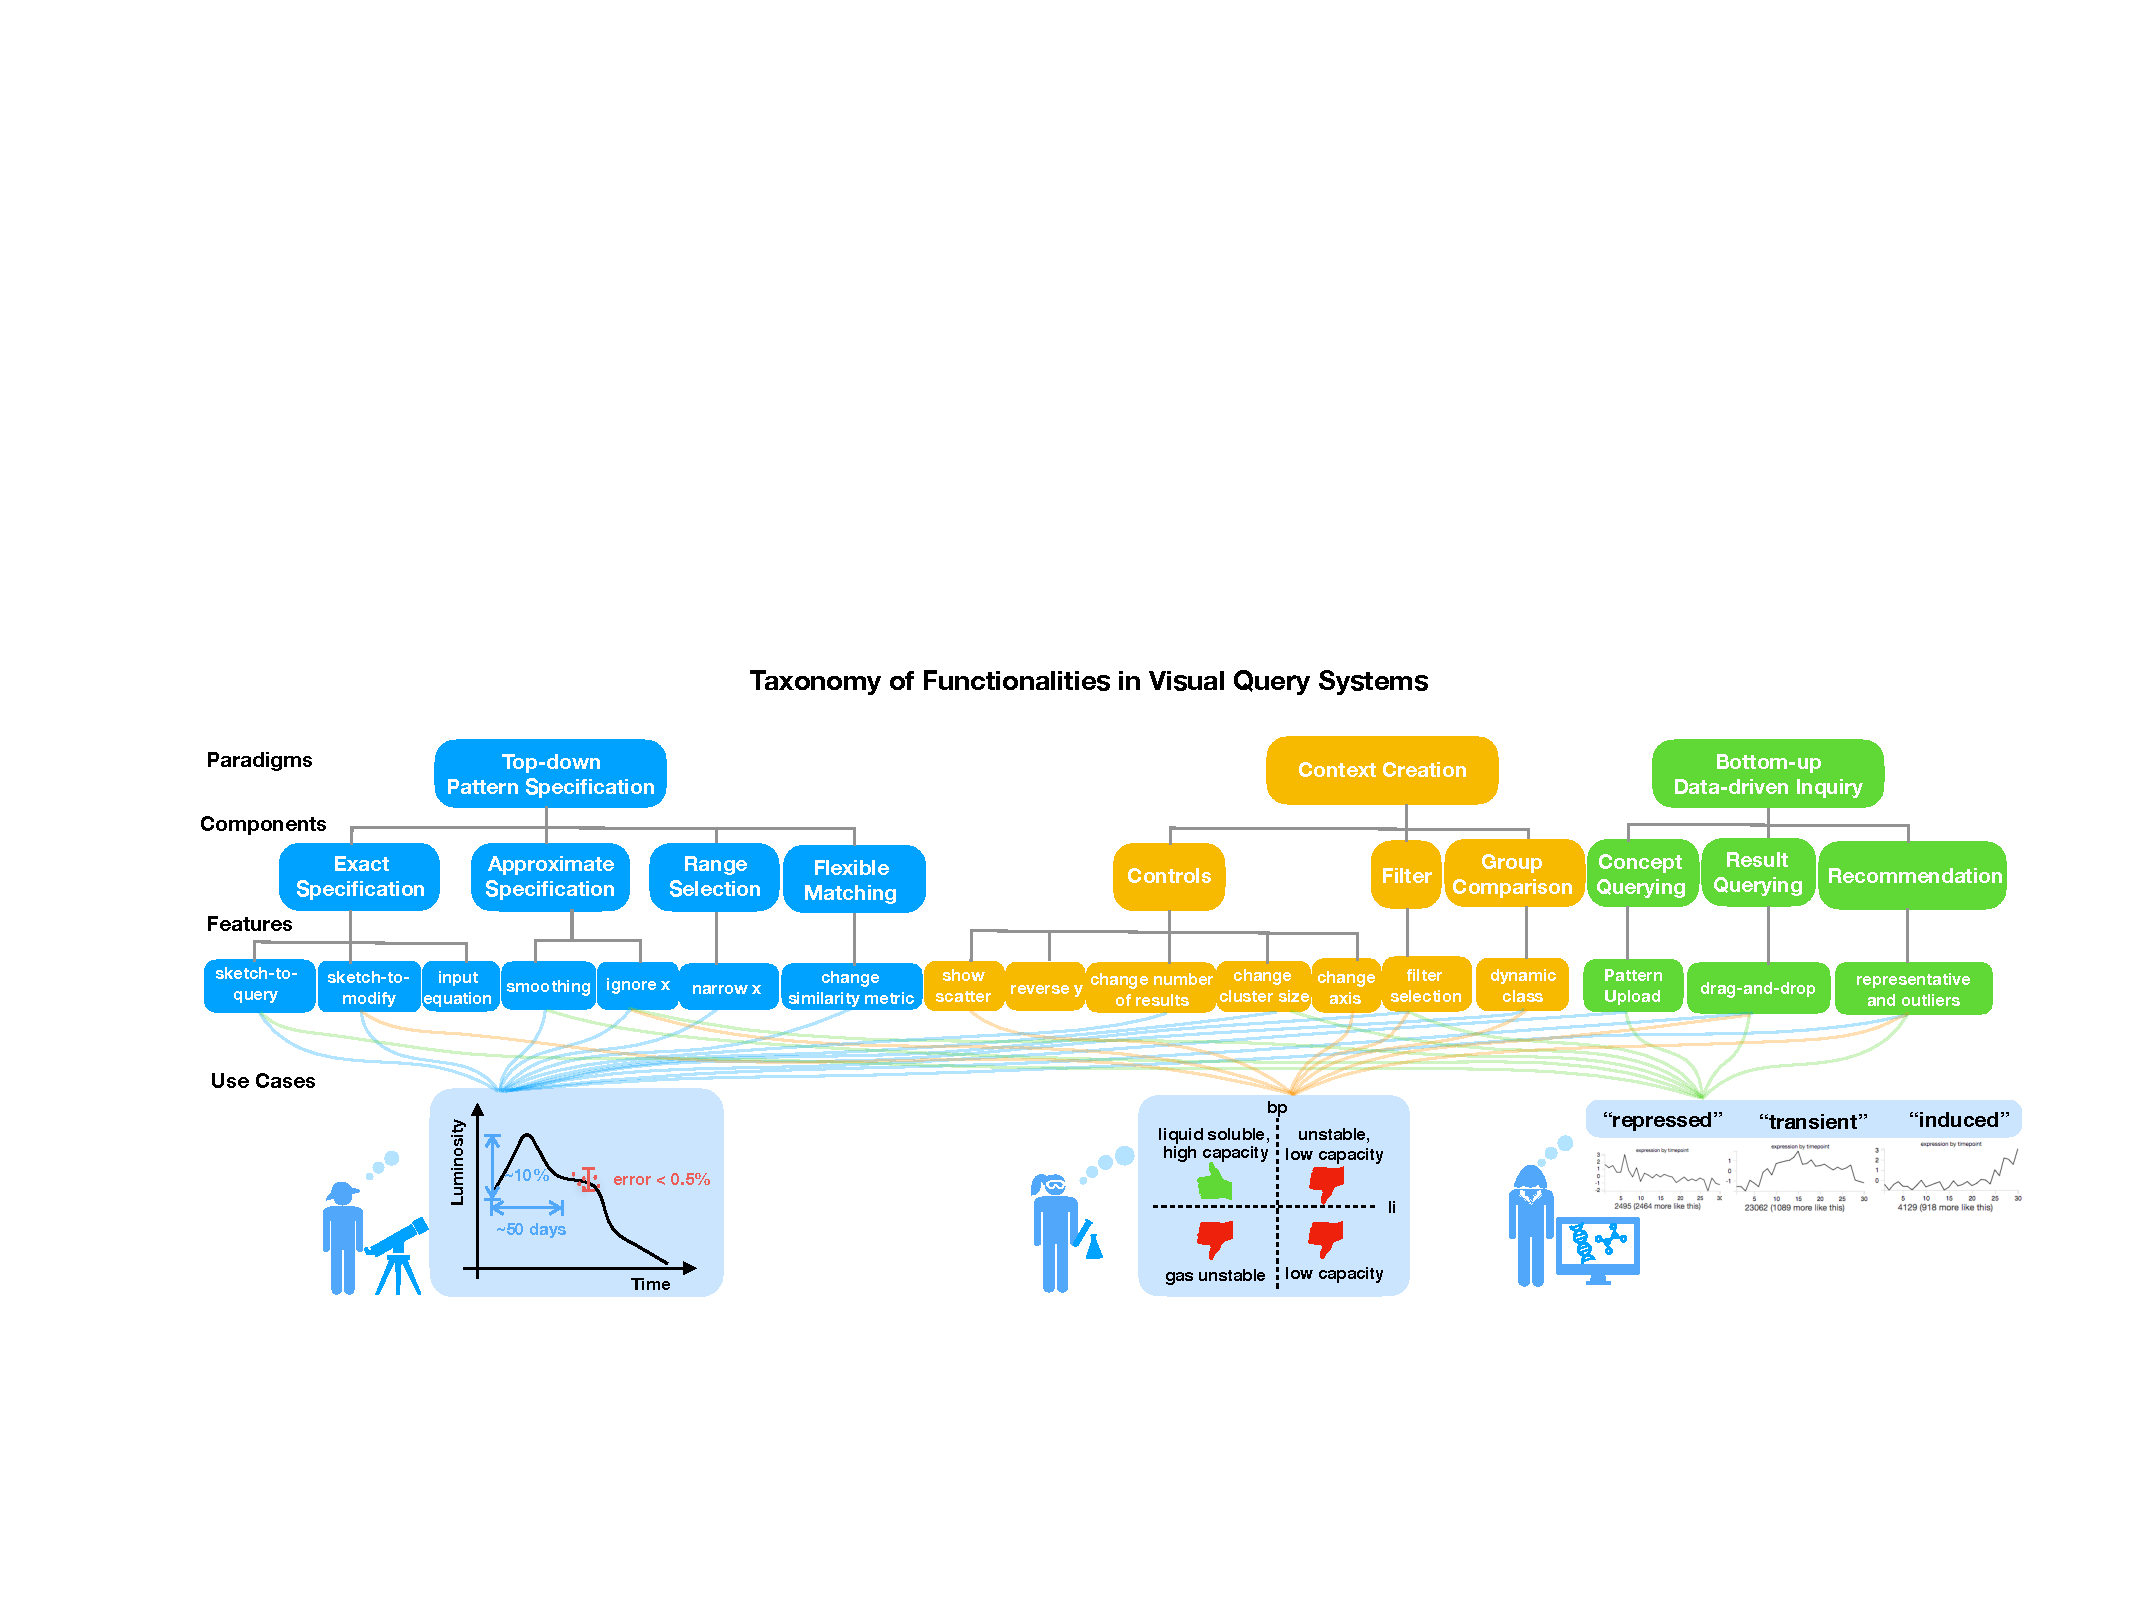
\includegraphics[width=\linewidth]{figures/full_taxonomy.pdf}
  \caption{Taxonomy of functionalities in VQSs. From top, each of the three paradigm is broken down into key components in the system, which is instantiated as features in \zv. The bottom-most layer connects the use cases features that have practical or envisioned usage based on the evaluation study.}
  \label{fig:taxonomy}
\end{figure*}
% \par Drawing from our participatory design experience, evaluation study, and literature review in this space, we design a taxonomy for understanding the key functionalities in VQSs. In Figure~\ref{fig:taxonomy}, we show how each use cases makes use of the different features in \zv, then we organize the features into key components for VQSs, which belongs to one of the three paradigms in the VQS design space.
In particular, we will describe the main form of inquiry addressed by each paradigm\cut{(\textit{what, where, which})}, the characteristic use case, and design challenges involved in building features that support these paradigms.
\boldpara{Top-down Pattern Specification:} Top-down approaches start with user's intuition about how their desired patterns should look like based on `theory', including visualizations from past experiences or an abstract conceptions based on external knowledge. The goal of top-down pattern specification is to address the \textit{which} questions in visual sensemaking (\textit{which pattern instance exhibits this pattern?}), effectively moving rightwards to the gray area in Figure~\ref{2dmodel} where the pattern instance is known.
\par Based on this preconceived notion of what to search for, the design challenge is to translate the query in the analyst's head to a query executable by the VQS. As shown in Figure~\ref{fig:taxonomy}, this includes both components for specifying the pattern as well as controls governing the underlying algorithm of how the shape-matching is performed. For example, A1 knows intuitively what a supernovae pattern looks like and the detailed constraints on the shape, such as the width and height of the peak as well as the level of signal-to-noise tolerance for defining a match. He performs exact specification through sketching, choses the option to ignore differences on the x axis, and changes the similarity metric for flexible matching.  %The design challenge of top-down pattern specification is to ----- enable users to How to translate the in-the-head query to visual query and how matching is done.
\boldpara{Bottom-up data-driven inquiry:} While the usage of each querying feature may vary from one participant to the next, generally, result querying and pattern upload are considered bottom-up approaches that go from data to theory by enabling users to query via examples of known visualizations. Bottom-up data-driven inquiries address the \textit{what} questions in the sensemaking process. For example, genetics participants do not have a preconceived knowledge of what to search for in the dataset. They were mostly interested in \textit{what types of patterns exist in the dataset} through representative trends and therefore queried mainly through these recommended results to jumpstart further queries. The goal of data-driven inquiry is to move towards the blue area in Figure~\ref{2dmodel} to help analysts gain more information about patterns of interest in-the-head.
% notion of what the pattern looks like
The design challenge of bottom-up approaches include designing the right set of `stimuli' that could provoke further data-driven inquiries, as well as low-effort mechanisms to search via these results.
\boldpara{Context Creation:} Analysts often navigate across different parts of the visualization subspace to narrow to a more manageable scope or to explore relationships between different visualization attributes. Context creation addresses the \textit{where} question of sensemaking by enabling analyst to pivot across different visualization collections. The goal is to learn about \textit{where the patterns of interest lies}, effectively moving upwards in Figure~\ref{2dmodel} along the known attributes region. For example, material scientists often do not start with a pattern in-the-head, but recognize salient trends such as inverse correlation or linear correlation. They switch between different visualized attributes or create different dynamic classes to study their data from different perspectives. The design challenge of context creation is to develop features that help navigate users to desired regions of the data, visualize and compare how the data changes between different contexts and ensure that the context is dynamically reflected across other functionalities in the VQSs.

% \par As illustrated in Figure \ref{fig:sbmodel}, our search-browse paradigm is motivated by the characteristic challenges and foraging acts each use cases pose on existing VQSs observed in our design study.
% \par In the astronomy use case, the participants knew the patterns they are looking for, but the patterns are hard to specify and find. The main challenge for the VQS involves finer specification of sketched patterns, such as amplitude and width of the peak and noise level tolerance for defining a pattern match. Describe more in D1. The main workflow for the astronomers in our user study involves \textit{enriching}, either through finer query specification or via filtering data subsets, to increase the probability that their queries would be more accurately matched with what they are looking for.

% %For example, G2 knew that there was three repeated measurements that was taken for every timestep, in one of the profiles there was a sharp jump whereas other datapoints are relatively flat, he then concludes by inspecting in the scatterplot view that the rise in gene expression is probably due to an experimental error rather than the activation of a gene, because the other two repeated measurements were similar in magnitude. In other words, the scatterplot view offered him density of points as another proxy to consider that was not offered in the line chart perspective.
%  %This is true for both participants with and without a desired pattern in mind. For the participant without a desired pattern (G2), he created groups based on quartile statistics of additional data attributes and recorded the most significant representative pattern.

% - What does the act of browsing and searching mean in the context of VQSs
%   - browse: viewing ranked result and any recommended results on the side, derived from the data and analysis context.
%   - search: act of going from a user's in-the-head concept to an actionable query that could be executed through the VQSs, most work have focussed on sketch, we allow more than this.
%   - The challenge of browsing and searching is well-known in information retrieval~\cite{Olston2003}, browse alone is limited by how much a user can browse and process at once, search alone can be ambiguous without sufficient context from looking at example results.
% \par Pirolli and Card's notional model further characterizes the trade-offs between three central activities in the information foraging process: exploring, enriching, and exploiting~\cite{Pirolli}.  We organize the features that we have developed in \zv into these foraging acts, as shown in Figure~\ref{feature_heatmap}.
% \par We find that participants often create unexpected workflows that chain together multiple analysis steps, including interactions, controls, and queries in order to address a higher-level research question. We find that participants often construct a central workflow, \tvcg{which they then iterate on while adding additional variations.} Their \emph{central workflow often resembles one of the three foraging acts} that aligns with the type of research question and dataset they are interested in. The variations are based on intermixing their central workflow with the other two foraging \tvcg{acts}.
% % We find that participants often have a strong inclination to perform tasks that resembles one of the three foraging act and sparsely intermixed with other activities to support their analysis, depending on the type of research question and dataset they are interested in.
% \par As illustrated in Figure \ref{fig:sbmodel}, our search-browse paradigm is motivated by the characteristic challenges and foraging acts each use cases pose on existing VQSs observed in our design study. For example, the genetics participants do not have a preconceived knowledge of what they want to search for in the dataset. They were mostly interested in \textit{exploring} clusters to gain an overall sense what profiles exist in the dataset \tvcg{through representative trends} and therefore queried mainly through drag-and-drop to jumpstart further queries. Point to need for D3 and D4. The variations to their main workflow include changing cluster sizes and display settings to offer them different perspectives on the dataset (\textit{exploit}) and filtering on data attributes (\textit{enriching}).
% \par In the astronomy use case, the participants knew the patterns they are looking for, but the patterns are hard to specify and find. The main challenge for the VQS involves finer specification of sketched patterns, such as amplitude and width of the peak and noise level tolerance for defining a pattern match. Describe more in D1. The main workflow for the astronomers in our user study involves \textit{enriching}, either through finer query specification or via filtering data subsets, to increase the probability that their queries would be more accurately matched with what they are looking for.
% \par The main workflow for material scientists involves \textit{exploiting}, since they spend the majority of their efforts performing ``close-reading'' of individual visualizations to understand the relationships between physical variables. The participants are able to identify interesting relationships between physical variables when they examine each closely, but they are not sure what patterns to look for to begin with. More in D2.
% %For example, G2 knew that there was three repeated measurements that was taken for every timestep, in one of the profiles there was a sharp jump whereas other datapoints are relatively flat, he then concludes by inspecting in the scatterplot view that the rise in gene expression is probably due to an experimental error rather than the activation of a gene, because the other two repeated measurements were similar in magnitude. In other words, the scatterplot view offered him density of points as another proxy to consider that was not offered in the line chart perspective.
%  %This is true for both participants with and without a desired pattern in mind. For the participant without a desired pattern (G2), he created groups based on quartile statistics of additional data attributes and recorded the most significant representative pattern.
% % [---] out of 9 of our participants had more than one main workflow.
